
\chapter{Instrukcja użytkownika}
\section{Początki pracy  z narzędziem}
Wtyczka pozwala na wygenerowanie formularza Google Forms z pliku kodującego w formacie JSON, automatyczne definiowanie jego treści na podstawie wstawek w \LaTeX{}'u oraz zarządzanie informacjami o tym, czy dany formularz przyjmuje przesyłane odpowiedzi. Na początek należy jednak pobrać i zainstalować zależności wykorzystywane przez narzędzie.
\subsection{Instalacja}
Na początku należy sklonować \href{https://github.com/agnpawicka/pracaInzynierska/}{repozytorium projektu} -- github.com/agnpawicka/pracaInzynierska.
\ind Następnie wejść w folder \textbf{source} i uruchomić plik o nazwie ,,install.sh''. Pozwoli to na zainstalowanie potrzebnych bibliotek.
\subsection{Praca z wtyczką}
Aby włączyć narzędzie należy uruchomić plik o nazwie ,,run.sh''. Uruchomi on lokalny serwer Node.js'owy oraz stronę internetową z interfejsem użytkownika.
\section{Schemat pliku kodującego (JSON)}
Poniżej znajduje się rozpisany schemat kodowania: 
\begin{figure}[H]
\begin{lstlisting}[language=json,firstnumber=1]
{"title": "string",
 "email": "string",
 "check": "boolean",
 "questions": {[{"type": "string", 
                 "text": "string",
                 "tex" : "boolean",
                 "answers": [{"answer" : "string",
                             "correct" : "boolean"}],
                 "points": "number"}]}
}

\end{lstlisting}
\end{figure}
Jest to opis tych wartości, które mogą być użyte - nie wszystkie są jednak  wymagane. Poniżej znajduje się szzegółowy opis pól i wartości:
\begin{itemize}
\item{title} - wartość tekstowa, odpowiada nagłówkowi formularza -  \textbf{pole wymagane},
\item{email} - adres e-mail edytora formularza (konieczne konto google) - \textbf{pole opcjonalne},
\item{check} - wartość boolowska mówiąca o tym, czy formularz ma udostępniać opcję automatycznego oceniania. Domyślna wartość to \textbf{false}. W przypadku ustawienia wartości na \textbf{true} należy się upewnić, że przy każdym pytaniu są poprawnie ustalone wartości ,,correct'' oraz ,,points'' - \textbf{pole opcjonalne},
\item{questions} - tablica, której każde pole zawiera informacje dotyczące jednego pytania - \textbf{pole wymagane}. Poniżej znajdują się wartości kodujące pojedyncze pytanie:
\begin{itemize}
\item{type} - pole tekstowe dotyczące typu kodowanego pytania. Dopuszczalne wartości:
\begin{itemize}
\item ,,checkBox'' - pytanie zamknięte wielokrotnego wyboru,
\item ,,grid'' - pytanie typu ,,prawda/fałsz'',
\item ,,list'' - zamknięte jednokrotnego wyboru,
\item ,,text'' - otwarte.
\end{itemize}
 \textbf{pole wymagane},
\item{text} - zawiera treść pytania w formie tekstowej. Może zawierać wstawki z \LaTeX{}'a. Należy jednak pamiętać, że JavaScript traktuje symbol ,,$\backslash$'' jako specjalny - wszystkie wystąpienia ,,$\backslash$'' należy więc zastąpić ,,$\backslash\backslash$'' - \textbf{pole wymagane},
\item{tex} - wartość boolowska, jeśli \textbf{true} treść pytania (text) będzie konwertowana do obrazu z zachowaniem konwersji symboli matematycznych i innych wstawek z \LaTeX{}'a z biblioteki standardowej, \textbf{pole wymagane},
\item{answers} - tablica, każde pole zawiera jedną z możliwych odpowiedzi w następującej formie:
\begin{itemize}
\item answer - pole tekstowe, treść danej odpowiedzi
\item correct - wartość boolowska wskazująca czy dana odpowiedź jest prawidłowa. Domyślna wartość: false.
\end{itemize} 
-\textbf{pole opcjonalne}
\item{points} - wartość numeryczna, odpowiada liczbie punktów przyznawanej za poprawą odpowiedź na pytanie (dotyczy wyłącznie oceniania automatycznego) - \textbf{pole opcjonalne}
\end{itemize}
\end{itemize}









\section{Obsługa narzędzia}
Po uruchomieniu użytkownik widzi stronę w przeglądarce, jak na zdjęciu poniżej:
\begin{figure}[H]
  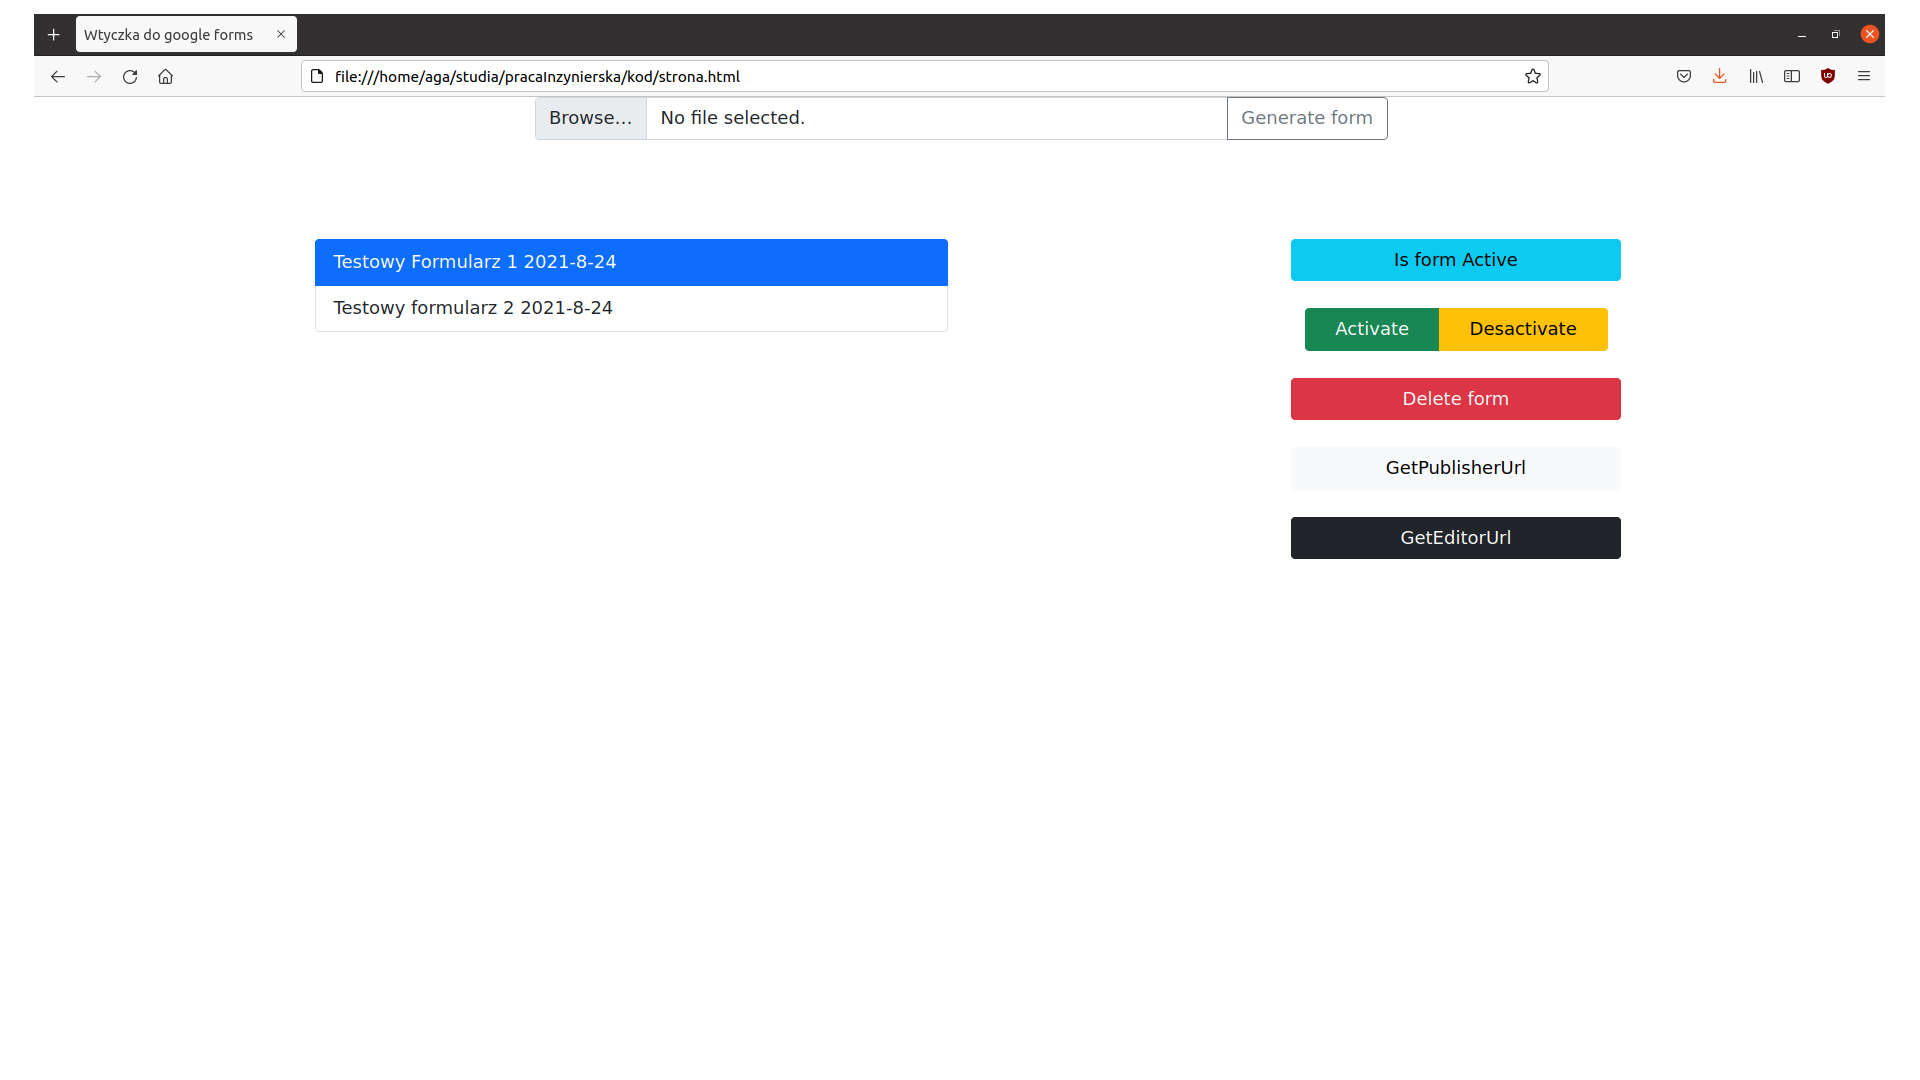
\includegraphics{strona.png}
  \caption{Interfejs aplikacji}
  \label{fig:1}
\end{figure}
\\Widoczne u góry pole do wgrywania plików przyjmuje formaty .txt oraz .json. W pliku powinien znajdować się zakodowany formularz (podrozdział 4.2. Schemat pliku kodującego (JSON)).
\\Poniżej  po lewej stronie znajduje się lista utworzonych już formularzy, po prawej znajdują się przyciski służące do operowania na już istniejących formularzach.
\\Przycisk ,,Generate form'' wgrywa podany plik i  wykonuje na nim kolejne operacje. Poprawne wykonanie powinno przechodzić przez kolejne etapy:
\begin{itemize}
\item Sprawdzany jest format  pliku. Jeśli zawartość jest obiektem typu JSON, dane przekazywane są do lokalnego serwera, w przeciwnym przypadku strona wyświetli alert informujący o niepoprawnym formacie.
\item Serwer lokalny sprawdza zgodność pliku ze schematem (JSON schema). Po tym etapie poniżej pola do wgrywania plików powinna pojawić się jedna z poniższych informacji:
\begin{itemize}
\item Validation succeded
\item Wrong JSON format
\end{itemize}
\item Jeśli plik JSON jest zgodny ze schematem, następuje konwersja pytań zakodowanych jako ,,tex'' na format zdjęciowy. 
\item Po zakończonej konwersji, z lokalnego serwera wysyłany jest POST request do serwera po stronie Google, gdzie odbywa się konwersja pliku na formularz. Zdalny serwer odsyła informację po zakończonej pracy do serwera lokalnego.
\item Lokalny serwer dodaje nowy formularz do listy.
\item Wyświetla się komunikat \textbf{New form has been created. Please reload the page} z prośbą o odświeżenie strony.
\end{itemize}
\ind Zachowania poszczególnych przycisków  - za wyjątkiem ,,Generate Form'' - dotyczą zawsze wybranego formularza z listy (podświetlonego w danym momencie na niebiesko). Aby wybrać formularz należy kliknąć na niego w liście formularzy. 
\ind Widoczne w interfejsie przciski mają następujące funkcje:
\paragraph{Is Form Active} zwraca wartość \textbf{Form is active} jeśli formularz przyjmuje odpowiedzi oraz \textbf{Form is inactive} w przeciwnym przypadku.
\paragraph{Activate} wysyła do serwera po stronie Google'a zapytanie, jeśli aktywacja formularza przebiegła pomyślnie, zwracana jest wiadomość \textbf{Form activated}.
\paragraph{Deactivate} wysyła do serwera po stronie Google'a zapytanie, jeśli dezaktywacja formularza przebiegła pomyślnie, zwracana jest wiadomość \textbf{Form deactivated}.
\paragraph{Delete Form} wysyła do serwera po stronie Google'a zapytanie o dezaktywnację formularza, następnie usuwa z pliku z danymi o formularzach wpis dotyczący wybranego formularza oraz w komunikacie \textbf{Form deactivated, please reload page.} prosi o odświeżenie strony
\paragraph{Get Publisher Url} wysyła do serwera po stronie Google'a zapytanie o adres url dla respondentów wybranego formularza. W komunikacie pojawia się odpowiedni link.
\paragraph{Get Editor Url} wysyła do serwera po stronie Google'a zapytanie o adres url dla edytorów wybranego formularza. W komunikacie pojawia się odpowiedni link.


